% Autor: Leonhard Segger, Alexander Neuwirth
% Datum: 2017-10-30
\documentclass[
	% Papierformat
	a4paper,
	% Schriftgröße (beliebige Größen mit „fontsize=Xpt“)
	12pt,
	% Schreibt die Papiergröße korrekt ins Ausgabedokument
	pagesize,
	% Sprache für z.B. Babel
	ngerman
]{scrartcl}

% Achtung: Die Reihenfolge der Pakete kann (leider) wichtig sein!
% Insbesondere sollten (so wie hier) babel, fontenc und inputenc (in dieser
% Reihenfolge) als Erstes und hyperref und cleveref (Reihenfolge auch hier
% beachten) als Letztes geladen werden!

% Silbentrennung etc.; Sprache wird durch Option bei \documentclass festgelegt
\usepackage{babel}
% Verwendung der Zeichentabelle T1 (Sonderzeichen etc.)
\usepackage[T1]{fontenc}
% Legt die Zeichenkodierung der Eingabedatei fest, z.B. UTF-8
\usepackage[utf8]{inputenc}
% Schriftart
\usepackage{lmodern}
% Zusätzliche Sonderzeichen
\usepackage{textcomp}

% Mathepaket (intlimits: Grenzen über/unter Integralzeichen)
\usepackage[intlimits]{amsmath}
% Ermöglicht die Nutzung von \SI{Zahl}{Einheit} u.a.
\usepackage{siunitx}
% Zum flexiblen Einbinden von Grafiken (\includegraphics)
\usepackage{graphicx}
% Abbildungen im Fließtext
\usepackage{wrapfig}
% Abbildungen nebeneinander (subfigure, subtable)
\usepackage{subcaption}
% Funktionen für Anführungszeichen
\usepackage{csquotes}
% Zitieren, Bibliographie
\usepackage{biblatex}
% Zur Darstellung von Webadressen
\usepackage{url}

% Verlinkt Textstellen im PDF-Dokument, hyperref und cleveref sollten (Reihenfolge auch hier
% beachten) als Letztes geladen werden!
\usepackage[unicode]{hyperref}
% "Schlaue" Referenzen (nach hyperref laden!)
\usepackage{cleveref}


% siunitx: Deutsche Ausgabe, Messfehler getrennt mit ± ausgeben
\sisetup{
	locale=DE,
	separate-uncertainty
}
\bibliography{6Mi_S2_25-10-2017_References}

\begin{document}
	
	\begin{titlepage}
		\centering
		{\scshape\LARGE Versuchsbericht zu \par}
		\vspace{1cm}
		{\scshape\huge S2 -- Experimentieren, und dann?\par}
		\vspace{2.5cm}
		{\LARGE Gruppe 6Mi \par}
		\vspace{0.5cm}
		
		{\large Alexander Neuwirth (E-Mail: a\_neuw01@wwu.de) \par}
		{\large Leonhard Segger (E-Mail: l\_segg03@uni-muenster.de) \par}
		\vfill
		
		durchgeführt am 25.10.2017\par
		betreut von\par
		{\large Christian} %TODO Nachname?
		
		\vfill
		
		{\large \today\par}
	\end{titlepage}
	\tableofcontents
	
	\newpage
	\section{Einführung}
	
	Der Ortsfaktor ist die Fallbeschleunigung, die sich aus Zentrifugalkraft (aufgrund der Erdrotation) und Erdanziehungskraft zusammensetzt. Sie kann für viele Anwendungen auf der Erdoberfläche als 9,81 \si{m/s^2} angenommen werden. Bei genauerer Betrachtung schwankt sie jedoch leicht, da sie abhängig von Höhe über NN, Breitengrad und Verteilung der Massendichte der Erde ist. Die Messung des Ortsfaktor im Physikalischen Institut in Münster ergab einen Wert zwischen 10,5 und 11 \si{m/s^2}. Dieser Wert liegt deutlich außerhalb der erwarteten lokalen Unterschiede. Dabei wurde die Zeit gemessen, die eine Metallkugel für eine feste Strecke vertikal zum Boden im freien Fall benötigt. Da dieser Wert eine große Abweichung von der Angabe der Physikalisch-Technischen Bundesanstalt hat (9,813 \si{m/s^2}), stellte sich die Frage, ob der Ortsfaktor für Münster angepasst werden muss.\par 
	Um entscheiden zu können, ob eine Änderung des Wertes notwendig ist, wurden mehrere Reproduktionsmessungen durchgeführt. Diese Messungen bestehen aus dem Bestimmen der Zeiten die Fadenpendel verschiedener Längen für eine Periode benötigen.  
	
	\section{Methoden}
	Um den Ortsfaktor mit einem Fadenpendel bestimmen zu können, haben wir die Formel für die Schwingdauer eines Fadenpendels verwendet.
		\begin{equation}\label{eq:Ortsfaktor}
			T_0 = 2\pi \sqrt{\frac{l}{g}}
			\Rightarrow{} g = 4\pi{}^2\frac{l}{T_0^2}
		\end{equation}
	Da diese Formel durch eine Kleinwinkelnäherung (\(\sin{\varphi} \approx \varphi \)) zustande kommt, gilt es zu beachten, dass man das Fadenpendel initial nicht zu weit auslenkt. %EDIT: Kleinwinkelnäherung ist--> aus einer zustande kommt
	Des Weiteren haben wir uns entschieden immer die Zeit für 20 Schwingungsperioden zu messen, da sich so der Reaktionsfehler zum Start und Ende der Messung reduzieren lässt. Die hängt damit zusammen, dass der Reaktionsfehler absolut ist und mit Zunahme der Schwingungsperioden nicht zunimmt, der Anteil des Fehlers an der Gesamtmessung also deutlich abnimmt.
	Als Anfangs- und Endpunkt unserer Messung haben wir die Ruhelage des Pendels gewählt. Für diesen Punkt haben wir uns entschieden, da sich das Pendel in diesem Punkt mit näherungsweise konstanter Geschwindigkeit bewegt und somit ist es leichter Reaktionsfehler auszugleichen. Ein alternativer Punkt wäre der Wendepunkt des Pendels gewesen, jedoch ist der exakte Zeitpunkt schwerer zu erkennen, da sich das Pendel langsamer bewegt und somit ist der Zeitraum, in dem das Pendel scheinbar stillsteht, groß und das Ende der Bewegung schwer genau zu erkennen.\par %EDIT: den Ort genommen, in dem sich das Pendel, wenn es nicht schwingt, befindet --> die Ruhelage (unnötig umständlich) + missing Kommas eingefügt + klarifiziert
	Sollten zusätzliche Schwingungen in andere Richtungen als die der initialen Auslenkung auftreten, so betrachten wir diese nicht weiter, da wir davon ausgehen, dass diese Schwingungen sich mit der zu messenden lediglich überlagern und sich die Gesamtschwingung wieder in die betrachtete Schwingung und eine senkrecht dazu stehende, keinen Einfluss auf die Messung habende, zweite Schwingung zerlegen lässt.
	\section{Ergebnisse}
	\subsection{Messungen}
	\subsubsection{Konstante Länge}
	Gemessen wurden 5 x 20 Schwingungen.
	\begin{itemize}
		\item Unsicherheit von \(l\): 
			\begin{itemize}
				\item $\pm0.5\si{cm}$ Abweichung, WDF Dreieck, Standardabweichung (Typ B): \( u_B(l) = \frac{1\si{cm}}{2\sqrt{6}} = 0.2\si{cm} \)
			\end{itemize}

		\item Unsicherheit von \(\bar{T}\): 
			\begin{itemize}
				\item Standardabweichung Mittelwert (Typ A): \( u_A(\bar{T}) = 0.0016\si{s} \)
				\item Reaktionszeit  $\pm0.19 \si{s}$, (Typ B): \( u_B(\bar{T}) = \frac{2\cdot0.19\si{s}}{2\sqrt{3}\cdot20} = 0.0055\si{s} \)
				\item Komb. Unsicherheit: $ u_C(\bar{T}) = \sqrt{(0.0016\si{s})^2+(0.0055\si{s})^2} = 0.0057 \si{s} $
			\end{itemize}
	\end{itemize}

	\begin{tabular}{l r}
		Länge des Pendels: & \(l = 114 \pm 0.2\si{cm} \) \\
		Mittelwert Schwingungsperiode: & \(\bar{T} = 2.1477 \pm 0.0057\si{s} \) \\
	\end{tabular} 
	

	\par

	\noindent Aus \eqref{eq:Ortsfaktor} folgt $ g = 9.757  \si{m/s^2}$. Die kombinierte Unsicherheit von g ergibt sich aus
	\begin{align*}
		u(g) = g * \sqrt{\left(\frac{u(l)}{l}\right)^2 + \left(2\frac{u(\bar{T})}{\bar{T}}\right)^2} = 0.055 \si{m/s^2} \\
		\Rightarrow{} g = (9.757 \pm 0.055) \si{m/s^2}
	\end{align*}
	


	\subsubsection{Verschiedene Längen}
	Gemessen wurden 2 x 20 Schwingungen bei 5 verschiedenen Längen $l$. \\
	In der Formel der Schwingperiode \eqref{eq:Ortsfaktor} ist ein wurzelförmiger Zusammenhang zwischen der Periode $T$ und dem Verhältnis $\frac{l}{g}$, deshalb sind in \cref{Messdaten} die Quadrate der Schwingungsperiode $T$ über $l$ aufgetragen. Aus den gemessenen Perioden ergab sich eine lineare Fitgerade mit der Steigung %EDIT: wurzelförmig klein + Verhältniss + desshalb
	\begin{equation*} 
		m = \frac{4\pi}{g} = \SI{4.0925 +- 0.0628 }{s^2/m}  
	\end{equation*}
	Die Unsicherheit $u(g)$ ergibt sich aus
	\begin{equation*}
		u(g) = 4\pi^2\frac{u_{\leq10}(m)}{m^2} = 4\pi^2t_{68}(3)\frac{u(m)}{m^2} = 0.18 \si{m/s^2}
	\end{equation*}
	und somit ergibt sich der Ortsfaktor  $g = \SI{9.65  +- 0.18}{m/s^2}$


	\begin{figure}[htb]
		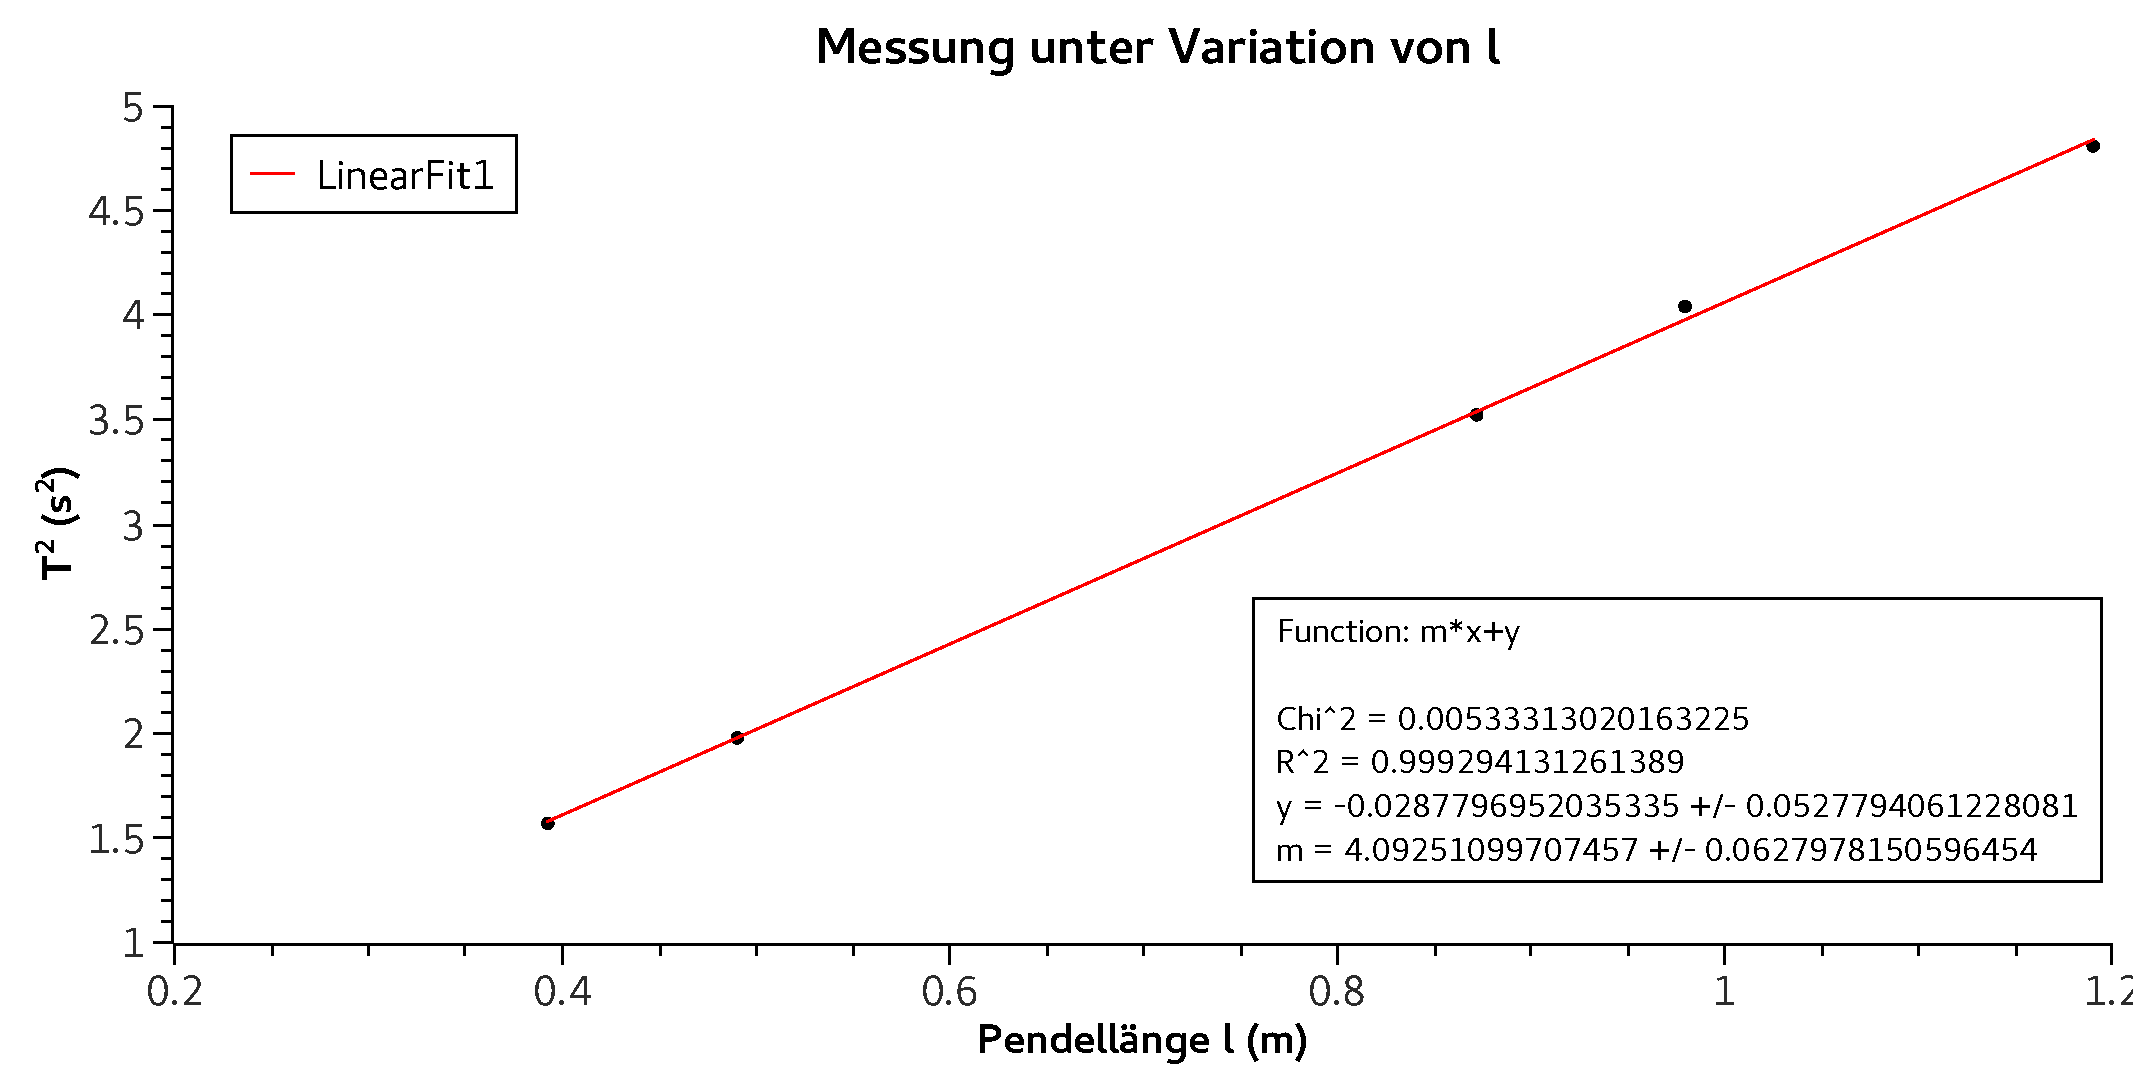
\includegraphics[width=1\textwidth]{Graph}
		\centering
		\caption{Messdaten Fadenpendel}
		\label{Messdaten}
		\centering
	\end{figure}

	Anmerkung: Die Fehlerbalken sind kleiner als die Symbole:
	\begin{itemize}
		\item $u(l)= 0.2 \si{cm} $
		\item $u(T^2) = 2 T u(T) = 0.0031 s \cdot T $
	\end{itemize}

	\subsubsection{Zusammenfassung der Ergebnisse}

	
	Der Ortsfaktor wurde von uns als $(9.757 \pm 0.055) \si{m/s^2}$ ermittelt. Die Angabe des PTBs (9.813 \si{m/s^2} ) liegt innerhalb der Abweichung des von uns ermittelten Wertes. Folglich unterstützen unsere Messungen die Literaturwerte und lassen auf keine der Erwartung widersprechende Fallbeschleunigung in Münster schließen.
	%EDIT Ich hab den Falltuŕm hier erst rausgelassen. Ist so eher eine reine Zusammenfassung unserer Ergebnisse. Mehr gibt's hier eigentlich nicht zu sagen.

	\section{Schlussfolgerung}
	Alles in allem ließen sich die Werte des Fallturm-Experiments nicht mittels eines Fadenpendels reproduzieren, denn sie liegen nicht innerhalb unserer Messunsicherheiten. Folglich ist davon auszugehen, dass die Ortsfaktorangabe der Physikalisch-Technischen Bundesanstallt nicht überdacht werden muss. Vorerst denkbar wäre auch eine lokale Beschränkung der Gravitationsanomalie auf den konkreten Raum der Messung. Dies wirkt bei genauerer Betrachtung jedoch unwahrscheinlich, da für die Schwankungen der Fallbeschleunigung auf der Erdoberfläche Zentrifugalkraft, Erdabplattung und Höhenprofil verantwortlich sind. Diese Faktoren ändern sich nicht merklich in unterschiedlichen Räumen eines Instituts. Außerdem schwankt laut einem Artikel in \enquote{Geophysical Research Letters} ~\cite[Abs. 12]{Fall} die Fallbeschleunigung auf der Erdoberfläche lediglich zwischen \SI{976392e-5}{m/s^2} und \SI{981974e-5}{m/s^2}. %TODO bibtex tut nicht, was es tun sollte. In den Folien vom Faschschaftsmenschen ging das so mit dem .bib-file.
	%Link zu Paper: http://onlinelibrary.wiley.com/doi/10.1002/grl.50838/full
	 Deshalb ist eine Abweichung, wie sie im Fallturm-Experiment gemessen wurde, unrealistisch.  Um die Gründe für die überraschende Messung der münsteraner Fallturm-Physiker herauszufinden, müsste mehr über die Rahmenbedingungen ihres Experiments und die Ungenauigkeiten ihrer Messung bekannt sein.


	%TODO Unsicherheiten hast du halt in Zusammenfassung der Ergebnisse gesagt. 

	%\bibliography{mybib} sollte man nicht brauchen und tut's bei mir auch nicht.
	%\bibliographystyle{standard}
	\printbibliography
\end{document}
